\section{Diode}
Eine Diode besteht aus PN übergängen und ist deswegen ein nichtlineares Element:
\begin{multicols}{2}
     \begin{minipage}{\linewidth}
         \begin{tabular}{ll}
             $ U_{DBR} $    & Durchbruchspanung  \\ 
             $ U_D $        & Diffusionsspannung (0.7V Si)  \\ 
             $ U_F $        & Flussspannung \\ 
             $ U_R $        & Sperrspannung  \\ 
              $ i_F $       & Diffusionsstrom, Strom in Durchlassrichtung  \\ 
              $ i_R $       & Leckstrom, Strom in Sperrichtung \\ 
            \end{tabular} 
        \end{minipage}
        
         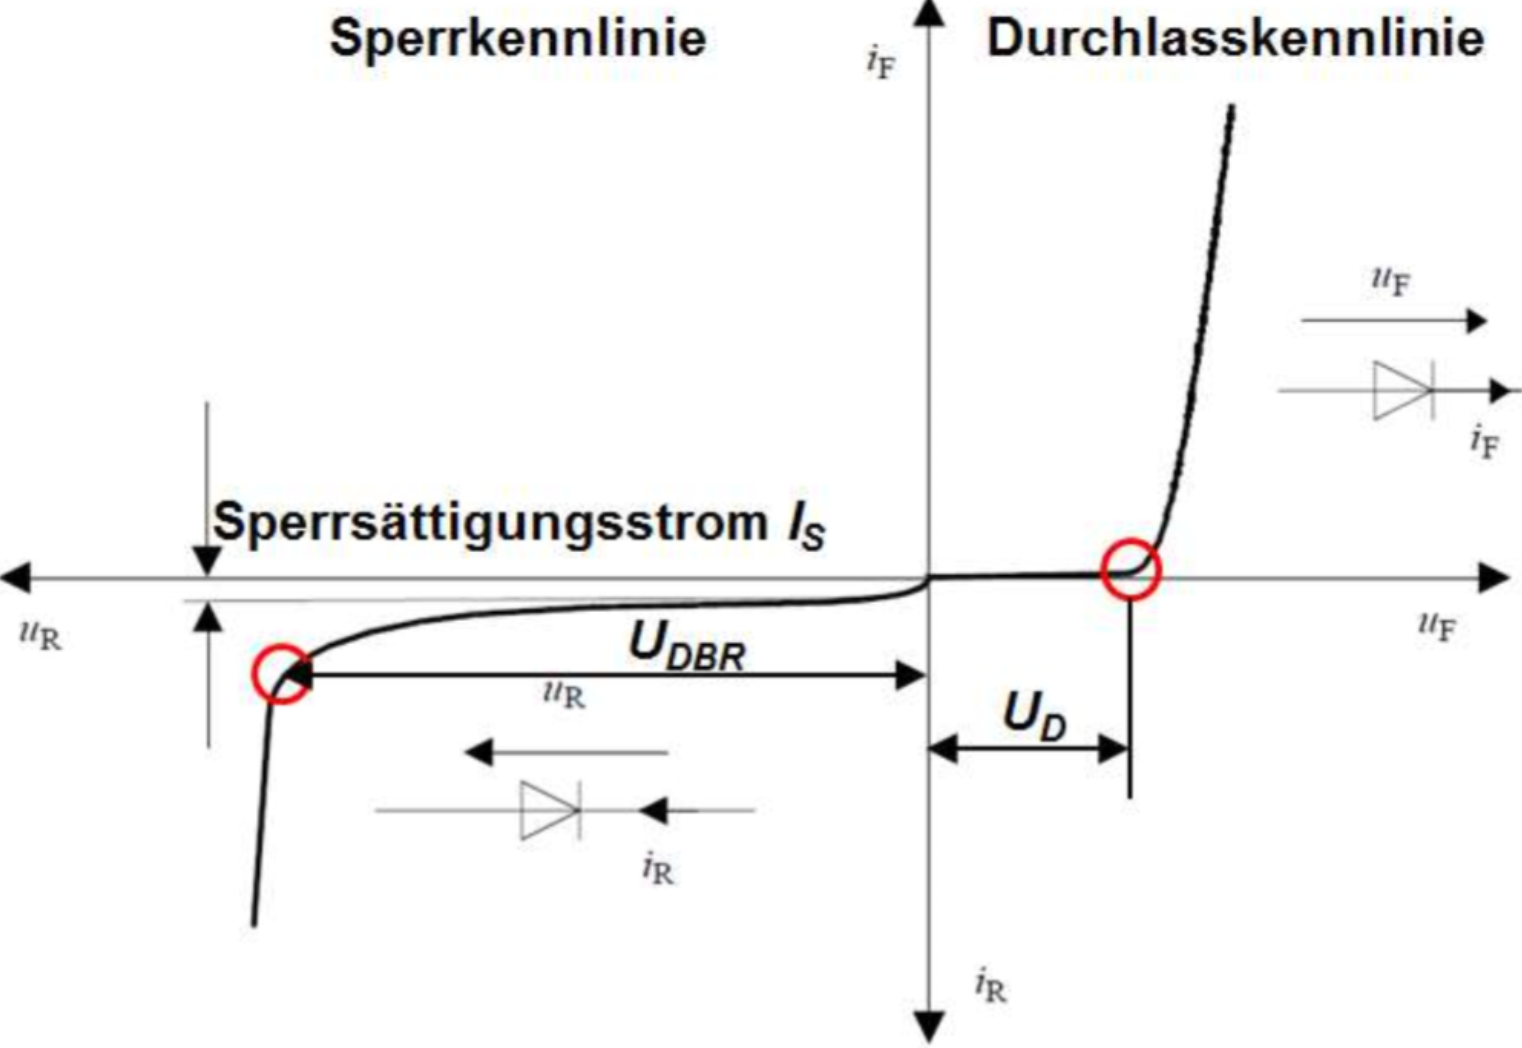
\includegraphics[width=0.8\linewidth]{images/kennlinieDiode}
\end{multicols}
\vspace{-1.5cm}
\begin{multicols}{2}
     \begin{minipage}{\linewidth}
         \begin{tabular}{ll}
             $ i_f ,\; u_F $& Durchlassrichtung\\
             $ U_{T0} $& Schwellenspannung\\
             $ r_f= \dfrac{\diff U_F}{\diff i_F} $& Differenzieller Durchlasswiderstand\\
            \end{tabular}       
    \end{minipage}
        
        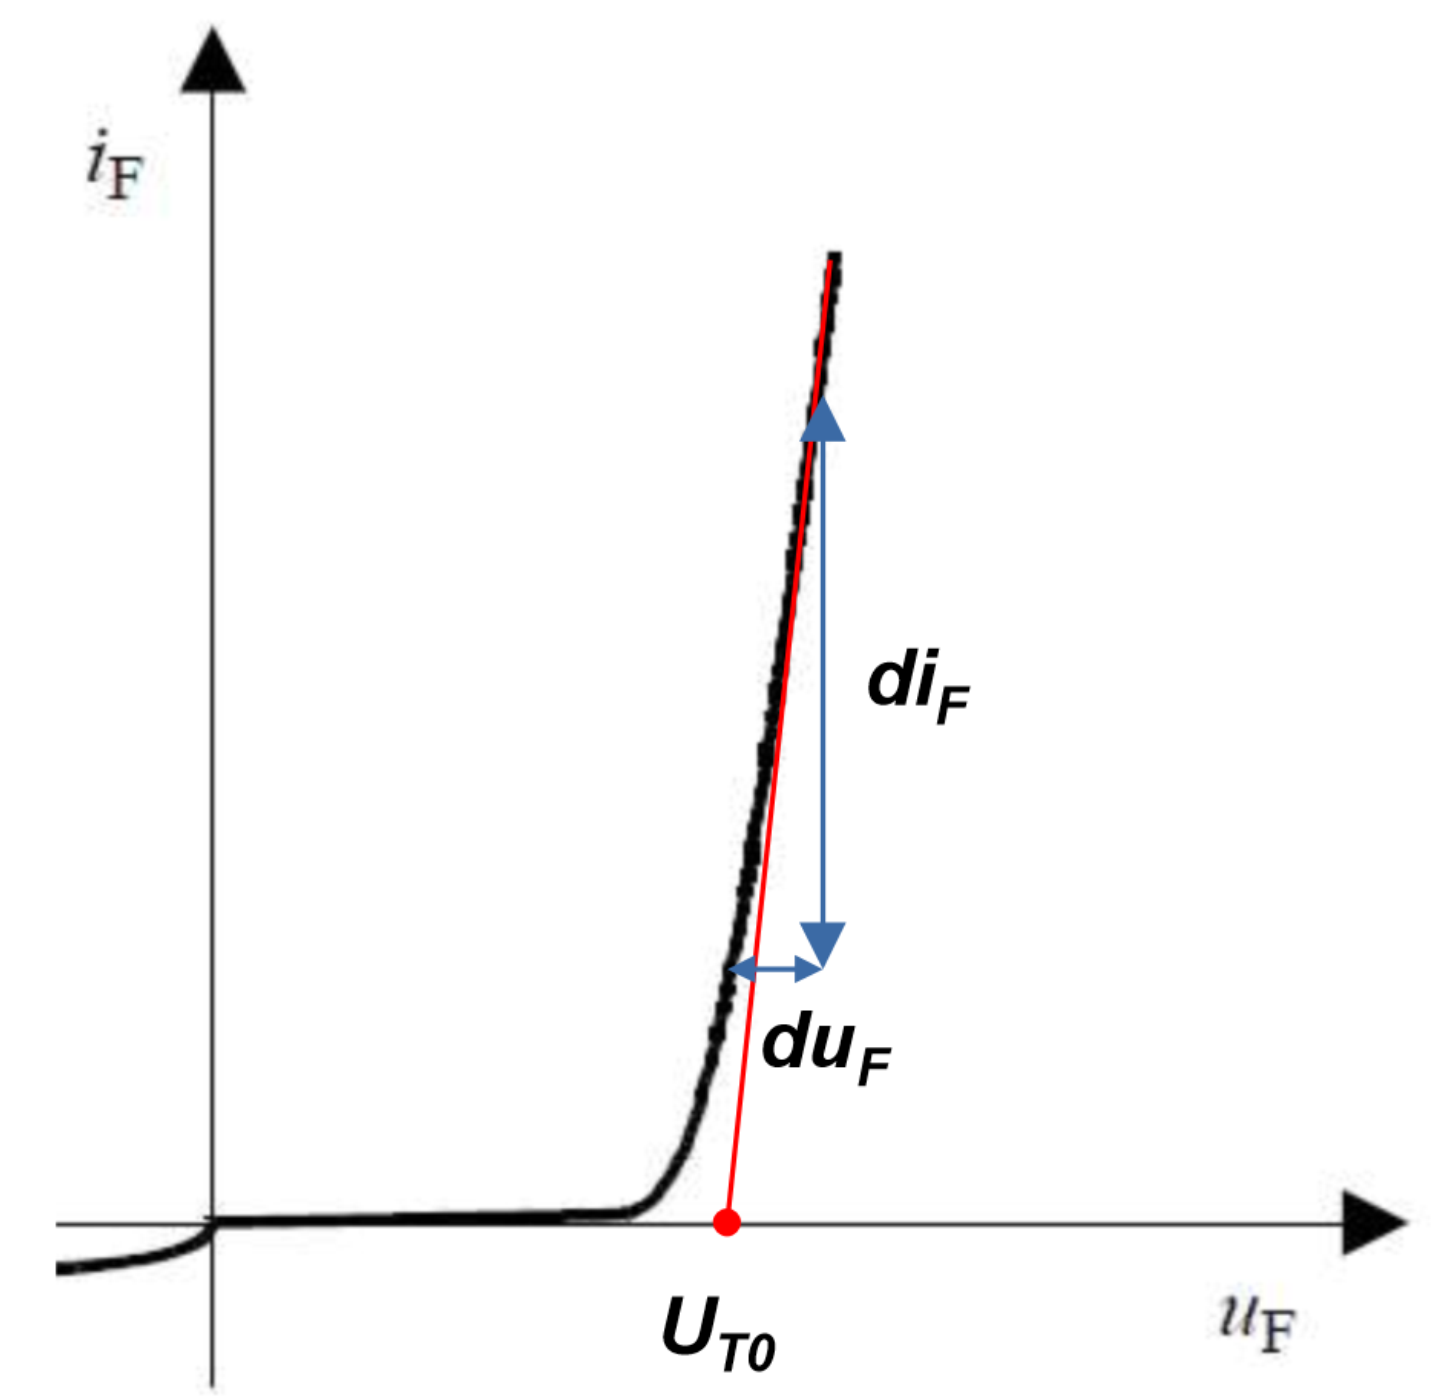
\includegraphics[width=0.4\linewidth]{images/dDiodeKennlinie}
\end{multicols}
\vspace{-1.5cm}
\subsection{Ersatzschaltbild}
\begin{multicols}{4}
    \begin{minipage}{\linewidth}
        \textbf{Reale Diode} \raggedright \newline\newline
        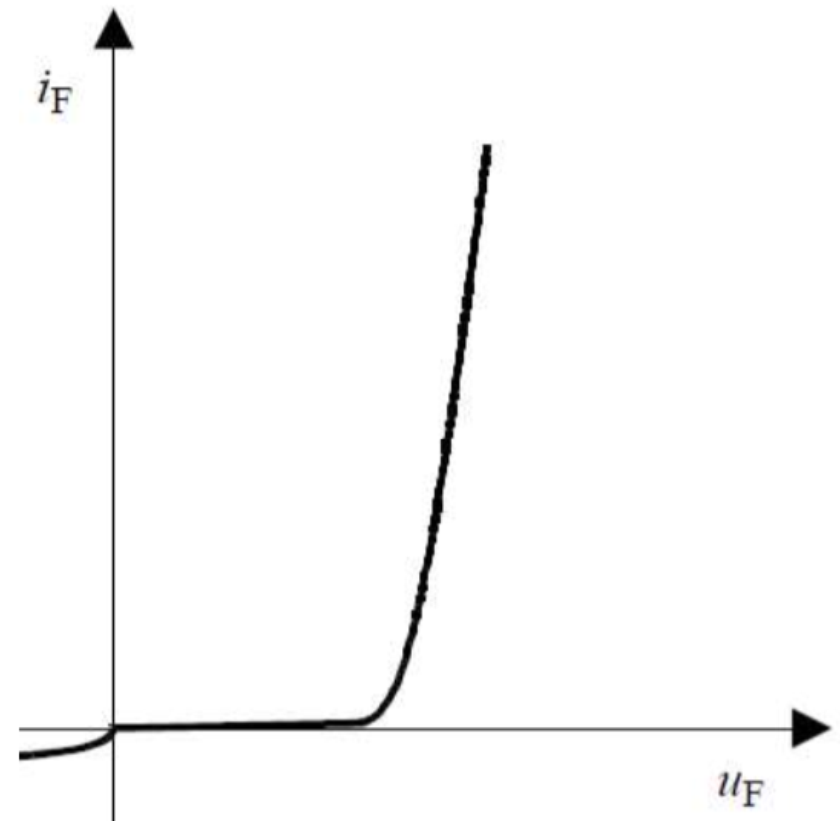
\includegraphics[width=0.7\linewidth]{images/realeDiode}
    \end{minipage}
    
    \begin{minipage}{\linewidth}
        \textbf{Ideale Diode ($ D_1 $)} \raggedright \newline\newline
        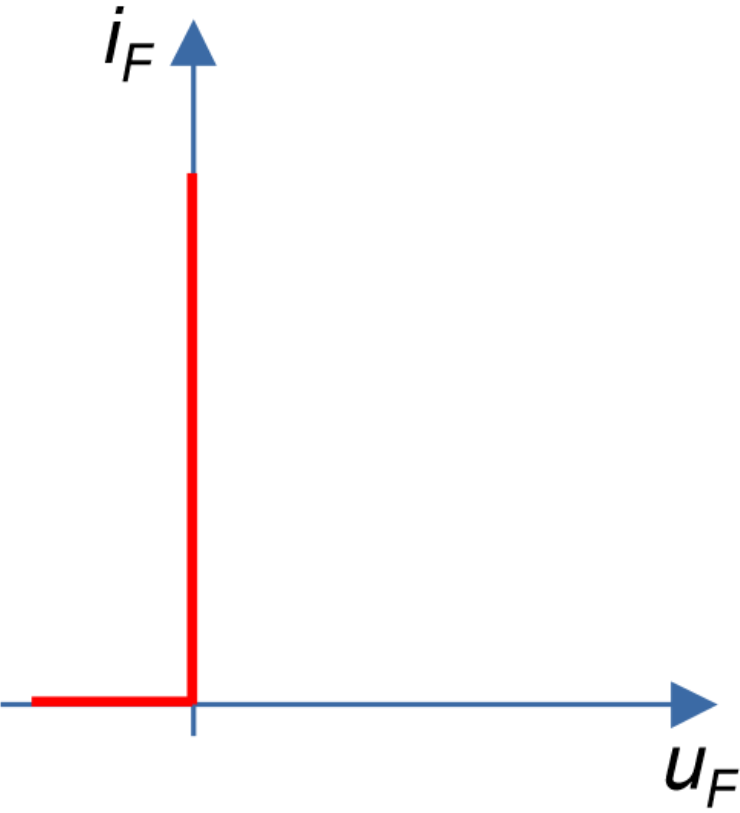
\includegraphics[width=0.7\linewidth]{images/idealeDiode}
    \end{minipage}
    
    \begin{minipage}{\linewidth}
        \textbf{Diode $ D_1 $ mit der Schwellenspannung $  D_2 $} \raggedright
        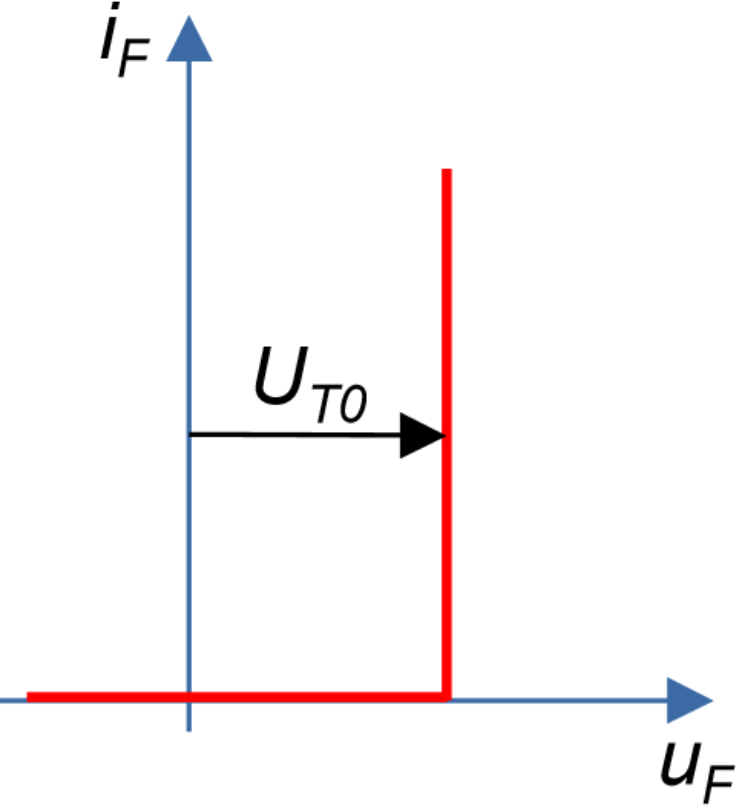
\includegraphics[width=0.6\linewidth]{images/idealeDiodeSP}
    \end{minipage}
    
    \begin{minipage}{\linewidth}
        \textbf{Diode $ D_2 $ mit dem Durchlasswiderstand($ D_3 $)} \raggedright
        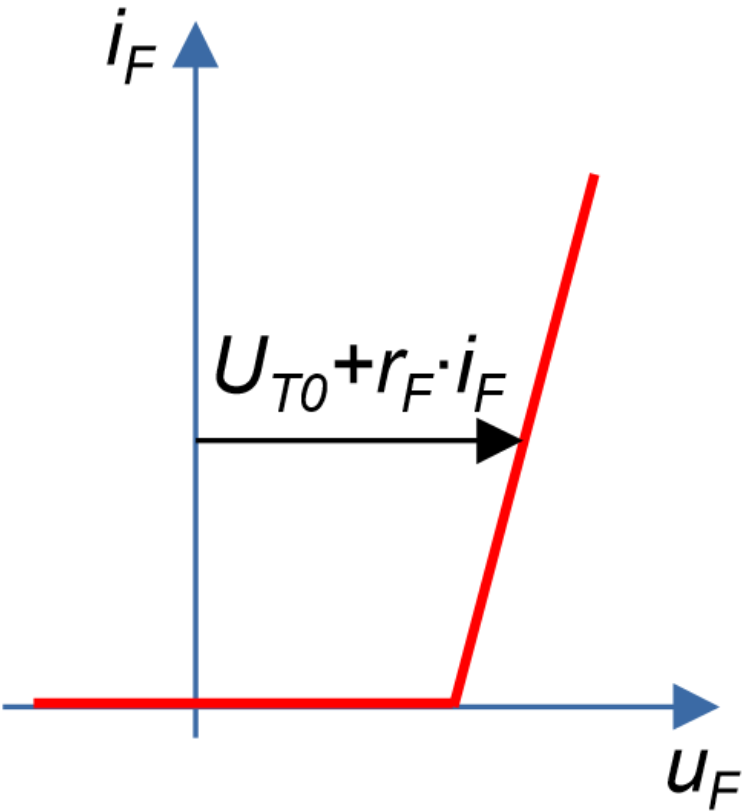
\includegraphics[width=0.6\linewidth]{images/idealeDiodeSPR}    
    \end{minipage}                       
\end{multicols}
\begin{multicols}{2}
\subsection{Grundformeln}
\begin{tabular}{ll}
    \textbf{Flussspannung}&\[ u_F = U_{T0} + i_F \cdot r_F \]\\
    \textbf{Momentanleistung}&\[ p(t)=u_F(t)\cdot i_F(t) \]\\
    \textbf{Verlustleistung}&\[ P_v=U_{TO}\cdot I_{FAV}+r_F\cdot I_{FRMS}^2 \]\\
    $ I_{FAV}$ & \qquad arithmetische Mittelwert von $ i_F $\\
    $ I_{FRMS} $ & \qquad Effektivwert von $ i_F $\\    
\end{tabular}

\hspace{1cm}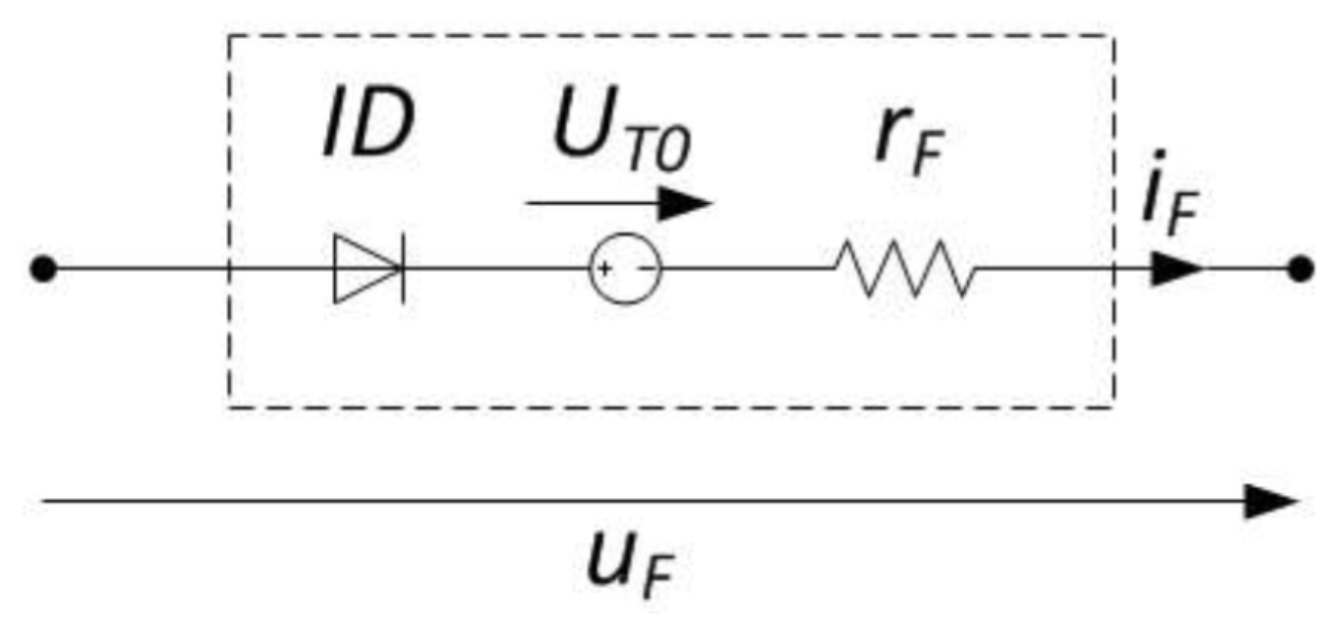
\includegraphics[width=0.6\linewidth]{images/ESBDiode} 
\end{multicols}

\subsection{Schaltverhalten und Schaltverluste}
    \begin{minipage}{0.7\linewidth}
        \raggedright
        \textbf{Durchlassverzug:}\newline
        freie Ladungsträger müssen zuerst die Ladungsfrei Zone "füllen"\newline\newline
        \textbf{Sperrverzug}\newline
        freie Ladungsträge müssen zuerst das Gebiet des pn-Überganges freiräumen\newline\newline
        Diese Erscheinungen sind wichtig bei  $\nicefrac{\diff u}{\diff t} > 100 \nicefrac{V}{\mu s} \; und \; \nicefrac{\diff i}{\diff t} > 10 \nicefrac{A}{\mu s} $
        \begin{tabular}{ll}
            $ I_{RM} $&Maximalwert des Rückstroms\\
            $ U_{RM} $&Maximalwert der Rückspannung\\
        \end{tabular}
    \end{minipage}   
    \begin{minipage}{0.3\linewidth}
        \vspace{-0.8cm}
        \raggedleft
            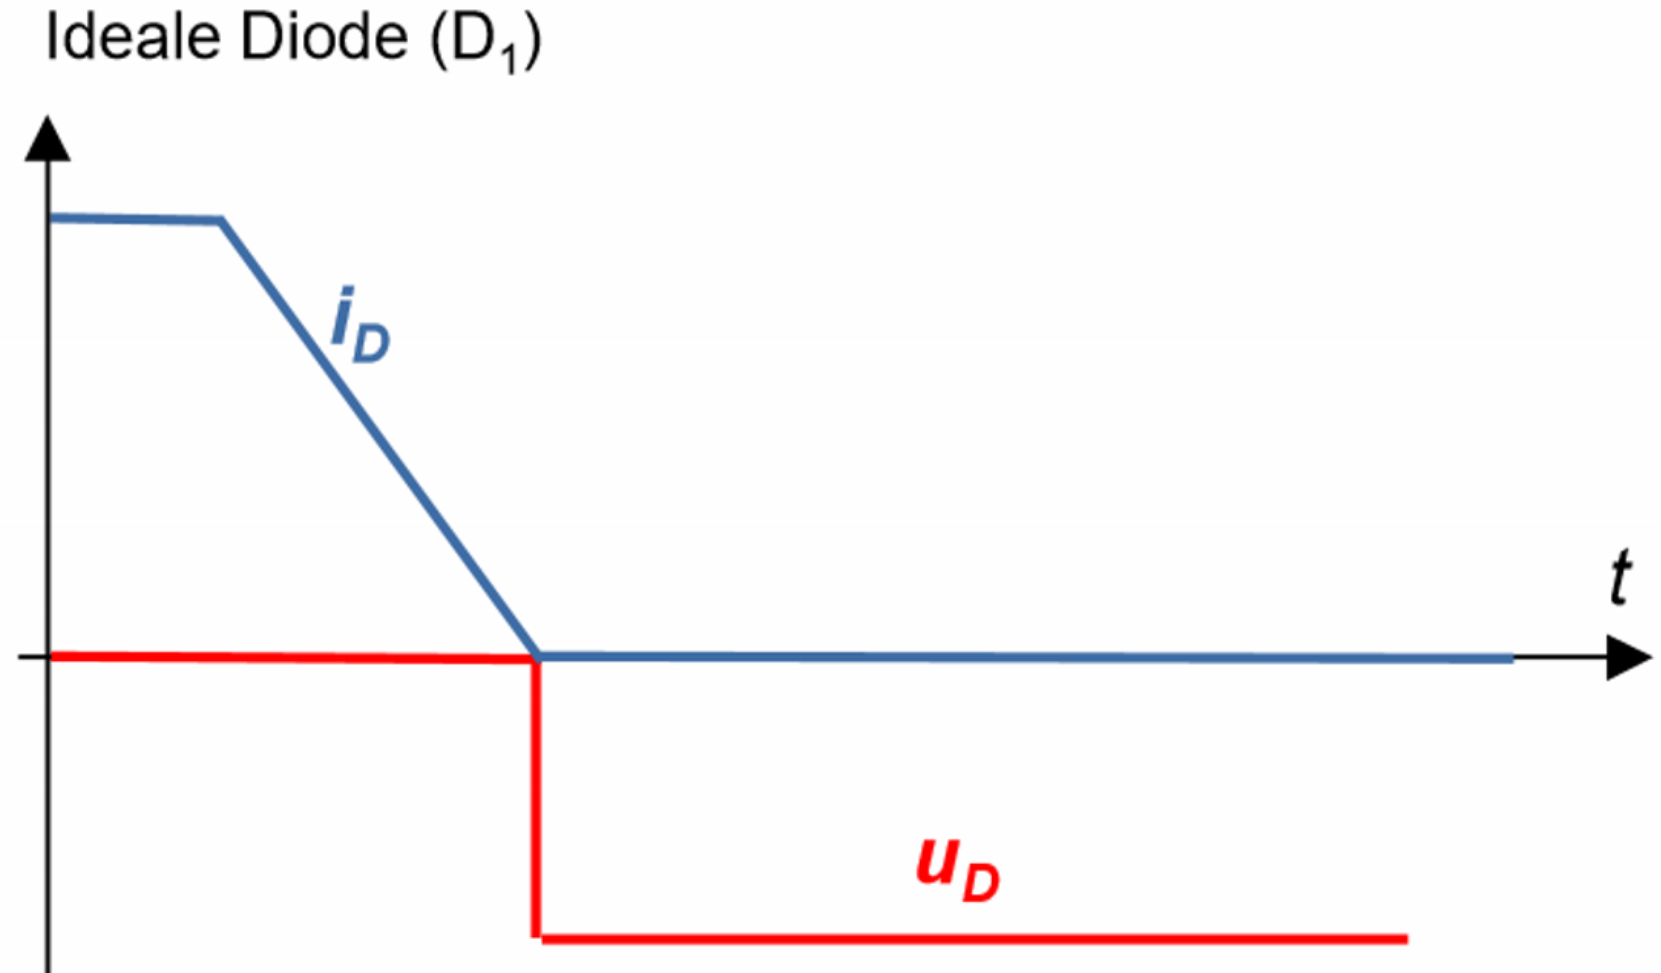
\includegraphics[width=\linewidth]{images/idealeDiodeSS}           
            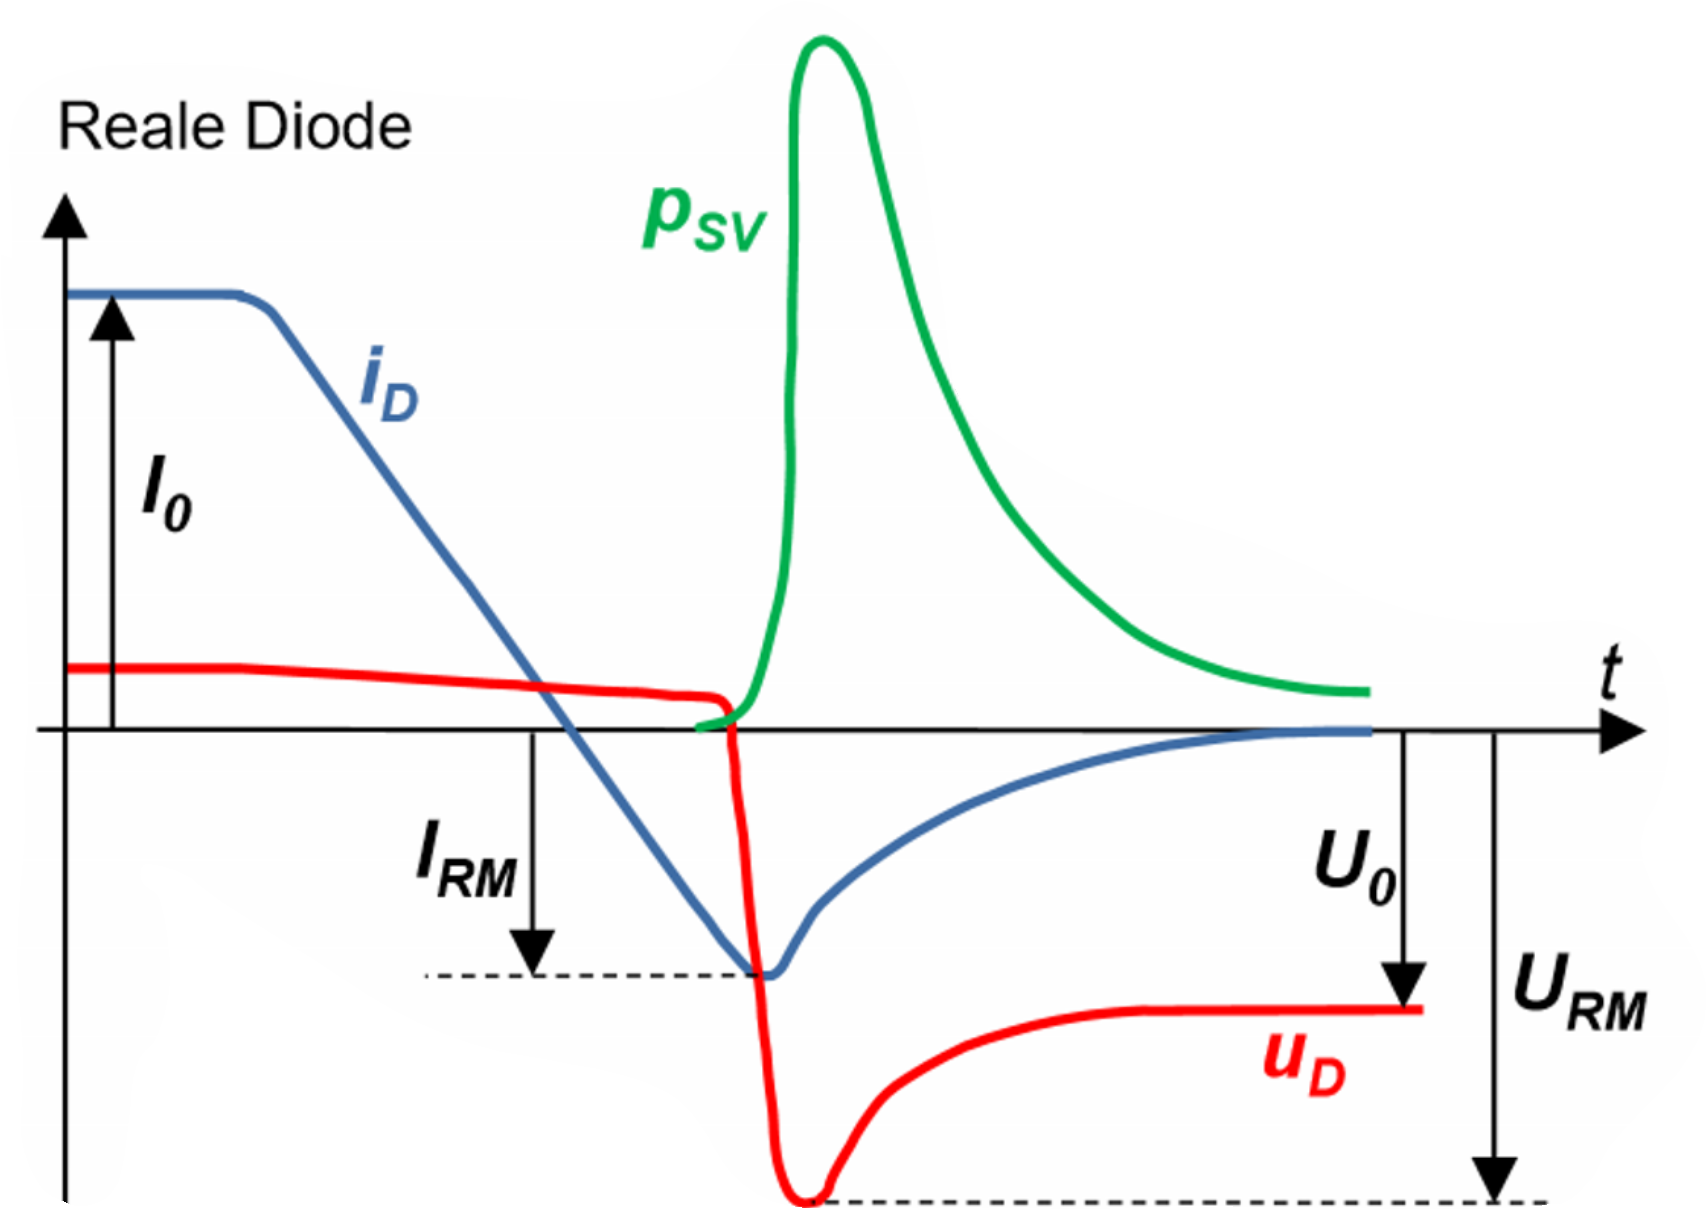
\includegraphics[width=\linewidth]{images/realeDiodeSS}
    \end{minipage}
\clearpage